\documentclass[a4paper,14pt]{extarticle}

\usepackage[utf8x]{inputenc}
\usepackage[T1,T2A]{fontenc}
\usepackage[russian]{babel}
\usepackage{hyperref}
\usepackage{indentfirst}
\usepackage{here}
\usepackage{array}
\usepackage{graphicx}
\usepackage{caption}
\usepackage{subcaption}
\usepackage{chngcntr}
\usepackage{amsmath}
\usepackage{amssymb}
\usepackage{pgfplots}
\usepackage{pgfplotstable}
\usepackage[left=2cm,right=2cm,top=2cm,bottom=2cm,bindingoffset=0cm]{geometry}
\usepackage{multicol}
\usepackage{askmaps}
\usepackage{titlesec}
\usepackage{listings}
\usepackage{color}
\usepackage{courier}

\definecolor{green}{rgb}{0,0.6,0}
\definecolor{gray}{rgb}{0.5,0.5,0.5}
\definecolor{purple}{rgb}{0.58,0,0.82}

\lstset{
	language=Verilog,
	backgroundcolor=\color{white},   
	basicstyle=\small\ttfamily,
	commentstyle=\color{green},
	keywordstyle=\color{blue},	
	numberstyle=\tiny\color{gray},
	stringstyle=\color{purple},
	breakatwhitespace=false,
	breaklines=true,
	captionpos=b,
	keepspaces=true,
	numbers=left,
	numbersep=5pt,
	showspaces=false,
	showstringspaces=false,
	showtabs=false,
	tabsize=4,
	frame=single,
	inputpath={../quartus/},
	literate={~} {$\sim$}{1}
}

\renewcommand{\le}{\ensuremath{\leqslant}}
\renewcommand{\leq}{\ensuremath{\leqslant}}
\renewcommand{\ge}{\ensuremath{\geqslant}}
\renewcommand{\geq}{\ensuremath{\geqslant}}
\renewcommand{\epsilon}{\ensuremath{\varepsilon}}
\renewcommand{\phi}{\ensuremath{\varphi}}
\renewcommand{\thefigure}{\arabic{figure}} 	
\renewcommand*\not[1]{\overline{#1}}

\titleformat*{\section}{\large\bfseries} 
\titleformat*{\subsection}{\normalsize\bfseries} 
\titleformat*{\subsubsection}{\normalsize\bfseries} 
\titleformat*{\paragraph}{\normalsize\bfseries} 
\titleformat*{\subparagraph}{\normalsize\bfseries} 

\counterwithin{figure}{section}
\counterwithin{equation}{section}
\counterwithin{table}{section}
\newcommand{\sign}[1][5cm]{\makebox[#1]{\hrulefill}}
\graphicspath{{../pics/}}
\captionsetup{justification=centering,margin=1cm}
\def\arraystretch{1.3}
\setlength\parindent{5ex}
\titlelabel{\thetitle.\quad}

\begin{document}

\begin{titlepage}
\begin{center}
	Санкт-Петербургский Политехнический Университет Петра Великого\\[0.3cm]
	Институт компьютерных наук и технологий \\[0.3cm]
	Кафедра компьютерных систем и программных технологий\\[4cm]
	
	\textbf{ОТЧЕТ}\\ 
	\textbf{по лабораторной работе}\\[0.5cm]
	\textbf{SystemVerilog №4}\\[0.1cm]
	Автоматизация проектирования\\ дискретных устройств\\[4.0cm]
\end{center}

\begin{flushright}
	\begin{minipage}{0.45\textwidth}
		\textbf{Работу выполнил студент}\\[3mm]
		группа 33501/4 \hspace*{9mm} Дьячков В.В.\\[5mm]
		\textbf{Преподаватель}\\[5mm]
		\sign[1.5cm] \hspace*{1mm} к.т.н., доц. Филиппов А.С. \\[5mm]
	\end{minipage}
\end{flushright}

\vfill

\begin{center}
	Санкт-Петербург\\
	\the\year
\end{center}
\end{titlepage}

\addtocounter{page}{1}
\counterwithin{lstlisting}{section}

\tableofcontents
\lstlistoflistings
\listoffigures
\newpage

\section{Цель}

\noindent Познакомиться с процедурой реализации проекта на базе процессора NIOSII.

\section{Выполнение работы}

\subsection{Создание аппаратной части проект помощью SOPC Builder}

Запустим в Qsys (Platform Designer) вкладку System Contents. Автоматически добавлен компонент source clock. 
\begin{figure}[H]
	\centering
	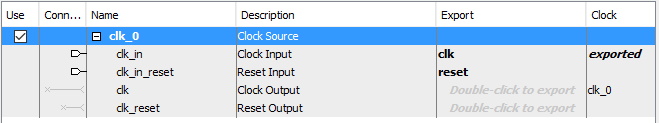
\includegraphics[scale=1]{1}
	\caption{System Contents}
\end{figure}

Зададим частоту тактового сигнала $25$ МГц.
\begin{figure}[H]
	\centering
	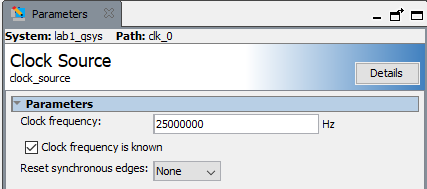
\includegraphics[scale=1]{2}
	\caption{Частота тактового сигнала}
\end{figure}

Создадим на основе встроенных модулей М9К память для команд и данных процессора.
\begin{figure}[H]
	\centering
	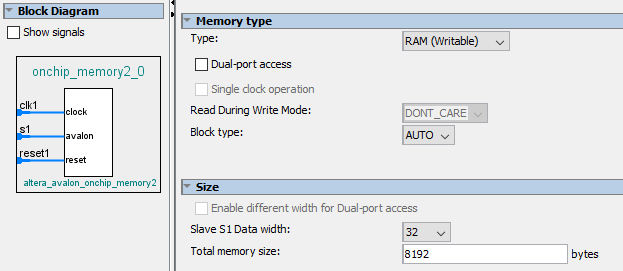
\includegraphics[scale=1]{3}
	\caption{Создание памяти для команд и данных процессора}
\end{figure}

Так как для нормальной работы компонент должен быть подключен к тактовому сигналу, сигналу сброса внутренних регистров и Мастеру на шине Avalon-ММ, то появились сообщения об ошибках и предупреждение.
\begin{figure}[H]
	\centering
	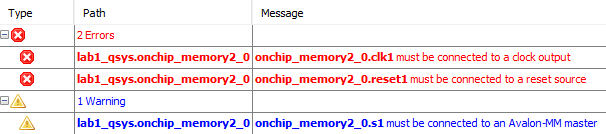
\includegraphics[scale=1]{4}
	\caption{Ошибки и предупреждение}
\end{figure}

Двойным щелчком в поле компонента откроем окно настройки и установим опцию Enable non-default initialization file (имя файла \code{onchip_mem.hex}).
\begin{figure}[H]
	\centering
	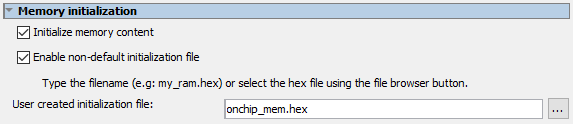
\includegraphics[scale=1]{5}
	\caption{Enable non-default initialization file}
\end{figure}

Соединим выход \code{clk} компонента \code{clk} с входом \code{clk1} компонента \code{onchip_mem}, а выход \code{clk_reset} компонента \code{clk} source с входом \code{reset1} компонента \code{onchip_mem}.
\begin{figure}[H]
	\centering
	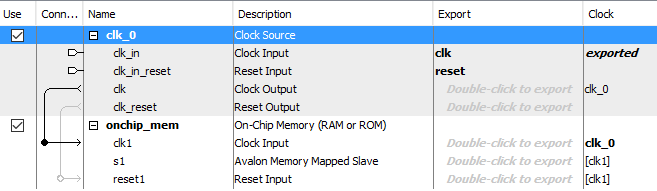
\includegraphics[scale=1]{6}
	\caption{Соединение компонентов}
\end{figure}

Сконфигурируем и подключим к системе ядра процессора NIOSII.
\begin{figure}[H]
	\centering
	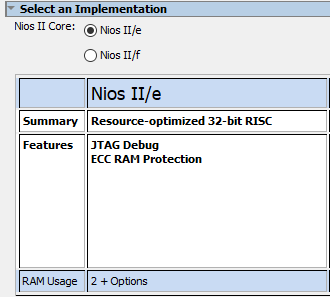
\includegraphics[scale=1]{7}
	\caption{Подключение к системе ядра процессора NIOSII}
\end{figure}

Соединим вход \code{clk} компонента \code{nios2_qsys} с выходом \code{clk1} компонента \code{clk}, а выход \code{clk_reset} компонента \code{clk} с входом \code{reset_n} компонента \code{nios2_qsys}. Соединим вход \code{s1} компонента \code{onchip_mem} с выходами \code{data_master} и \code{instruction_master} компонента \code{nios2_qsys}.
\begin{figure}[H]
	\centering
	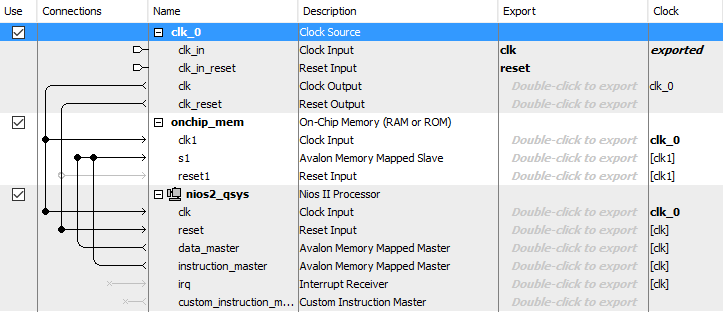
\includegraphics[width=\linewidth]{8}
	\caption{Соединение компонентов}
\end{figure}

На закладке Core NiosII укажем память для вектора сброса и вектора exception:
\begin{figure}[H]
	\centering
	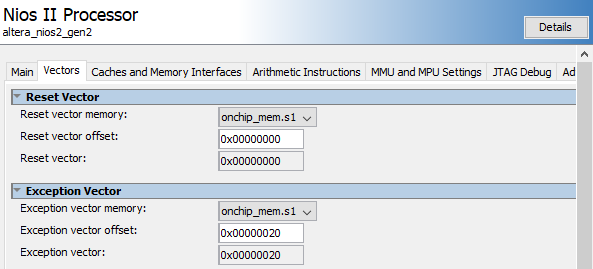
\includegraphics[scale=1]{9}
	\caption{Память для вектора сброса и вектора exception}
\end{figure}

Сконфигурируем и подключим к системе модуль PIO.
\begin{figure}[H]
	\centering
	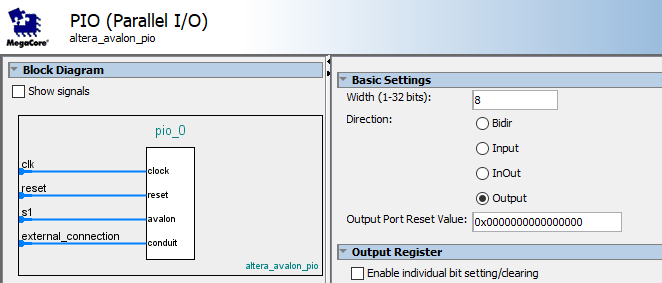
\includegraphics[width=\linewidth]{10}
	\caption{Подключение к системе ядра модуля PIO}
\end{figure}

Соединим вход \code{clk} компонента \code{pio} с выходом \code{clk1} компонента \code{clk}, а выход \code{clk_reset} компонента \code{clk} с входом \code{reset} компонента \code{pio}. Соединим вход \code{s1} компонента \code{pio} с выходами \code{data_master} и \code{instruction_master} компонента \code{nios2_qsys}.
\begin{figure}[H]
	\centering
	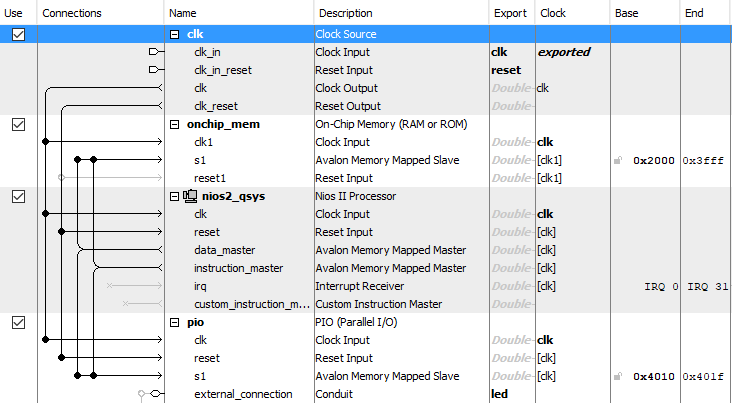
\includegraphics[width=\linewidth]{11}
	\caption{Соединение компонентов}
\end{figure}

Внешний вид созданной системы, закладка Address Map.
\begin{figure}[H]
	\centering
	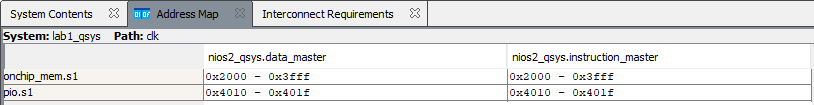
\includegraphics[width=\linewidth]{12}
	\caption{Address Map}
\end{figure}

Закладка Messages содержит одно предупреждение, информирующее о том, что не подключен JTAG Debug модуль.
\begin{figure}[H]
	\centering
	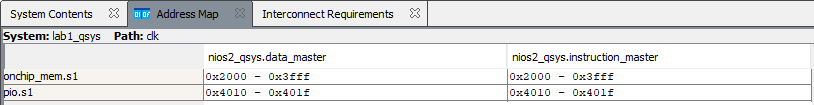
\includegraphics[scale=1]{13}
	\caption{Messages}
\end{figure}

\subsection{Интеграция аппаратной части проекта}

Создадим в графическом редакторе файл верхнего уровня в иерархии проекта и введем схему.
\begin{figure}[H]
	\centering
	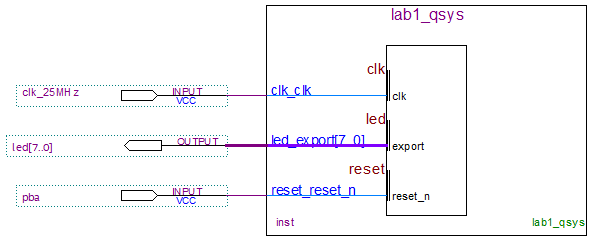
\includegraphics[scale=1]{14}
	\caption{\code{lab1.bdf}}
\end{figure}

Подключим файл с описанием созданной в Qsys системы к проекту.
\begin{figure}[H]
	\centering
	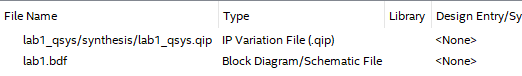
\includegraphics[scale=1]{15}
	\caption{Подключение описания к проекту}
\end{figure}

Назначим выводы проекта.
\begin{figure}[H]
	\centering
	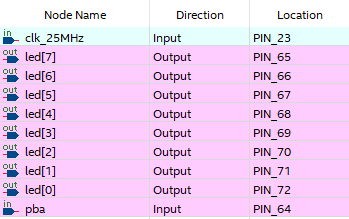
\includegraphics[scale=1]{16}
	\caption{Pin Planer}
\end{figure}

Интеграция аппаратной части проекта и задание установок проекта завершено.

\subsection{Создание программной части проекта в рамках оболочки NIOSII IDE}

Запустим оболочку для разработки/отладки программ -- NIOSII IDE.
\begin{figure}[H]
	\centering
	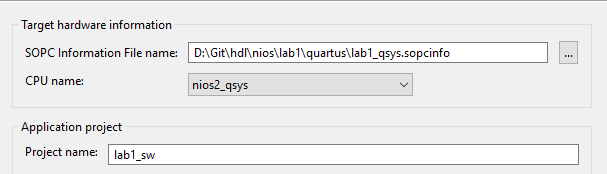
\includegraphics[scale=1]{17}
	\caption{NIOSII IDE}
\end{figure}

Создадим файл \code{lab1_source.c}.
\begin{figure}[H]
	\centering
	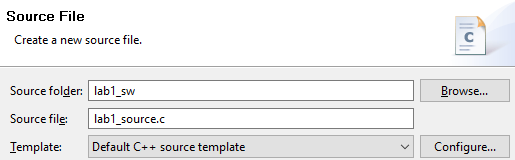
\includegraphics[scale=1]{18}
	\caption{Pin Planer}
\end{figure}

В листинге \ref{code:1} приведен код на языке C.
\lstinputlisting[caption=\code{lab1_source.c}, label=code:1]{software/lab1_sw/lab1_source.c}

Выставим основные настройки в BSP Editor.
\begin{figure}[H]
	\centering
	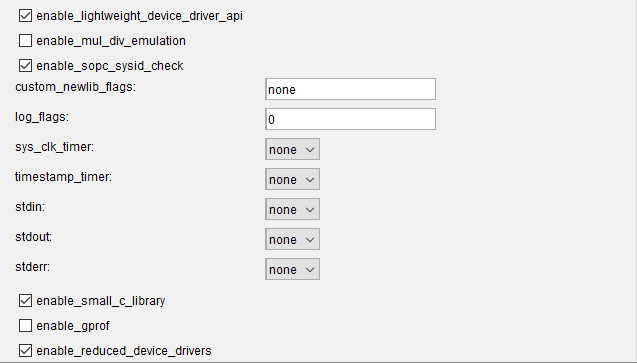
\includegraphics[scale=0.9]{19}
	\caption{BSP Editor}
\end{figure}

Запустим компиляцию проекта и генерацию файлов инициализации.
\begin{multicols}{2}
\begin{figure}[H]
	\centering
	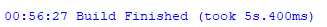
\includegraphics[scale=0.9]{20}
	\caption{Компиляция проекта}
\end{figure}
\begin{figure}[H]
	\centering
	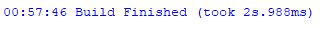
\includegraphics[scale=0.9]{21}
	\caption{Генерация файлов инициализации}
\end{figure}
\end{multicols}

Компиляция программы закончена успешно. Создан \code{onchip_mem.hex} файл для инициализации модуля памяти программ процессора.

\subsection{Полная компиляция проекта}

Добавим к проекту файл \code{meminit.qip} и запустим полную компиляцию проекта.
\begin{figure}[H]
	\centering
	
\includegraphics[scale=1]{22}
	\caption{Компиляция проекта}
\end{figure}
\begin{figure}[H]
	\centering
	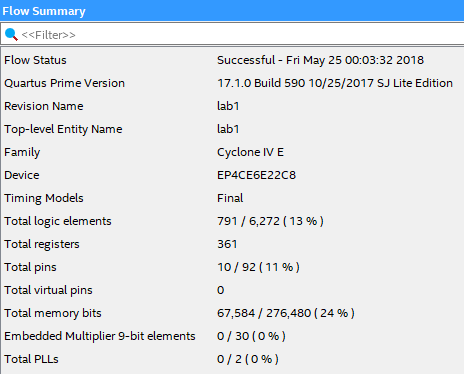
\includegraphics[scale=1]{23}
	\caption{Аппаратурные затраты}
\end{figure}

\subsection{Проверка проекта на стенде}

Подключим плату к компьютеру и выполним загрузку программы на плату. На плате загораются светодиоды, отображая 8-разрядные числа от 0 до 255 с частотой около 2 Гц (2 значения в секунду). Программа работает правильно.

\section{Выводы}

В ходе данной работы были изучены основы построения проекта на базе процессора NIOSII. Сначала был создан проект в QII и настроена аппаратная часть с помощью SOPC Builder, затем аппаратная часть была интегрирована в проект как объект symbol в файл .bdf. Программная часть проекта была создана с помощью NIOSII IDE на языке C. После подключения программной части была выполнена полная компиляция проекта и его проверка на плате. 

\end{document}